% !TEX root =  ../main.tex
\section{LazySpread}
\subsection{Definition}

\subsubsection{Signature} \cstr{lazySpread(s : set<VM>)}

\begin{itemize}
\item \cstr{s} : a set of at least 2 VMs for a meaningful constraint. VMs not in the \st{Running} state are ignored.
\end{itemize}

The \cstr{lazySpread} constraint forces all the running VMs in \cstr{s} to be hosted on distinct servers at the end of a reconfiguration process.

\classification{lazySpread}{application administrator}{VM placement}{VM-to-VM placement,Fault tolerance,Partitioning}

\subsubsection{Usage}

The \cstr{lazySpread} constraint may be used by an application administrator to provide to a replicated service, fault tolerance to hardware failures. By hosting each replicas on a distinct server, the service will  be
available while at least one server is still online. To achieve this purpose, one \cstr{lazySpread} constraint can
be used with the replicas provided as arguments.

\subsubsection{Example}

Figure~\ref{fig: lazySpread} depicts a sample reconfiguration between a source and a destination
configuration. In this example, the following \cstr{lazySpread} constraints were considered:


\begin{reconfiguration}
\centering
\begin{minipage}[b]{0.40\textwidth}
\begin{lstlisting}
N1: VM1 VM2
N2: VM4
N3: VM3
\end{lstlisting}
\end{minipage}
\begin{minipage}[b]{2cm}
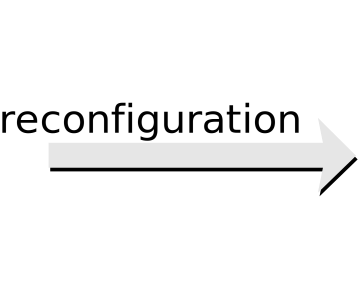
\includegraphics[width=2cm]{img/arrow_reconfiguration}
\end{minipage}
\begin{minipage}[b]{0.40\textwidth}
\begin{lstlisting}
N1: VM1
N2: (VM4) VM3
N3: VM2
\end{lstlisting}
\end{minipage}
\caption{A reconfiguration motivated by \cstr{lazySpread} constraints.}\label{fig: lazySpread}
\end{reconfiguration}

\begin{itemize}

\item \cstr{lazySpread(\{VM1, VM3, VM4\})}. This constraint was satisfied in the sour\-ce configuration as each VM were running on distinct servers. The constraint is still satisfied in the destination configuration despite \cstr{VM3} and \cstr{VM4} are colocated as \cstr{VM4} has been suspended.

\item \cstr{lazySpread(\{VM1,VM2\})}. This constraint was not satisfied in the source configuration as both VMs where running on \cstr{N1}. The relocation of \cstr{VM2} to \cstr{N3} fixed this violation.

\item \cstr{lazySpread(\{VM2, VM3\})}. This constraint was satisfied in the source configuration as both VMs were running on distinct servers. The constraint is still satisfied in the destination configuration despite the relocation of \cstr{VM2} to \cstr{N3} that was running \cstr{VM3} initially as \cstr{VM3} has been relocated elsewhere to let both VMs be running on distinct servers at the end of the reconfiguration process.
\end{itemize}


\fullVersion{
\subsection{Model}

This constraint is modeled using a negations between the d-slice placement variables of the running VMs.

\begin{equation*}
\begin{split}
\forall V \subseteq \mathcal{V}, \ lazySpread(V) \triangleq&\\
   & \forall v_i,v_j \in V, d_i^h \neq d_j^h
\end{split}
\end{equation*}

\subsection{Violation Detection}

The detection of the violating elements in \cstr{lazySpread} consists in identifying VMs that are hosted
on a same server. When a server hosts multiple VMs that are involved in the \cstr{lazySpread}
constraints, it is ensured that at least one VM is misplaced. Such a violation detection is however not guarantee to be optimal as it is not possible to know exactly which of the colocated VMs are supposed to be hosted elsewhere.

\subsection{Availability}
\subsubsection{In {\btrp}} 
This constraint is available in {\btrp} since the version 2.0 using the name \texttt{LazySpread}.
Using the global constraint catalog, the assigned for each of the d-slice placement variable is
ensured to be unique  using one \emph{allDifferent}~\cite{allDiff} global constraint.

\begin{equation*}
\begin{split}
\forall V \subseteq \mathcal{V}, \ lazySpread(V) \triangleq&\\
   & \text{\em allDifferent}(\forall d_i^h | v_i \in V)
\end{split}
\end{equation*}

\subsubsection{In VMWare DRS} 

The \emph{VM to VM} affinity rule may disallow a set of VMs to share servers.
}

\subsection{See also}

\subsubsection{Related Constraints}
\begin{itemize}
\item \cstrref{gather}: the opposite constraint of \cstr{spread}
\item \cstrref{spread}: a constraint similar to \cstr{lazySpread}
but which also guarantee that the VMs will never overlap on a same server, even during the reconfiguration process.
\end{itemize}

\emulatedWith{lazySpread}{split}{\cstr{lazySpread(s)}}{\cstr{split(s/\card{s})}}
\emulatedWith{lazySpread}{mostlySpread}{\cstr{lazySpread(s)}}{\cstr{mostlySpread(s,\card{s})}}
\emulatedWith{lazySpread}{splitAmong}{\cstr{lazySpread(s1)}}{\cstr{splitAmong(s/\card{s},\allNodes/\card{\allNodes})}}
\printListOfInheritance{lazySpread}